\documentclass{article}
\usepackage[utf8]{inputenc}
\usepackage{minted}
\usepackage{courier}
\usepackage[T1]{fontenc}
\usepackage[latin9]{inputenc}
\usepackage{amsmath}
\usepackage{amssymb}
\usepackage{graphicx}
\usepackage[unicode=true,
 bookmarks=false,
 breaklinks=false,pdfborder={0 0 1},backref=section,colorlinks=true]
 {hyperref}
\makeatletter
\usepackage{geometry}
\usepackage{xcolor}
\geometry{a4paper,left=2cm,right=2cm,top=1cm,bottom=1cm}

\title{Python Code}
\author{rj1407 }
\begin{document}

\section{3.1 Feature Normalization}
\begin{minted}[mathescape,
               linenos,
               numbersep=5pt,
               gobble=2,
               frame=lines
               framesep=2mm]{csharp}
  def feature_normalization(train, test):
    """Rescale the data so that each feature in the training set is in
    the interval [0,1], and apply the same transformations to the test
    set, using the statistics computed on the training set.

    Args:
        train - training set, a 2D numpy array of size (num_instances, num_features)
        test - test set, a 2D numpy array of size (num_instances, num_features)

    Returns:
        train_normalized - training set after normalization
        test_normalized - test set after normalization
    """
    # TODO
    #discard features that are constant in the training set
    feature_removal = np.std(train, axis=0) != 0
    train1 = train.transpose()
    train = train1[np.where(feature_removal)].transpose()
    test1 = test.transpose()
    test = test1[np.where(feature_removal)].transpose()
    
    #feature normalization
    MIN = np.amin(train,axis=0)
    MAX = np.amax(train,axis=0)
    train_normalized = (train - MIN)/(MAX - MIN)
    test_normalized = (test - MIN)/(MAX - MIN)
    return train_normalized, test_normalized
\end{minted}

\section{3.2 Gradient Descent Setup}
\subsection{3.2.5}
\begin{minted}[mathescape,
               linenos,
               numbersep=5pt,
               gobble=2,
               frame=lines
               framesep=2mm]{csharp}
  def compute_square_loss(X, y, theta):
    """
    Given a set of X, y, theta, compute the average square loss for predicting y with X*theta.

    Args:
        X - the feature vector, 2D numpy array of size (num_instances, num_features)
        y - the label vector, 1D numpy array of size (num_instances)
        theta - the parameter vector, 1D array of size (num_features)

    Returns:
        loss - the average square loss, scalar
    """
    #TODO
    loss = 0 #Initialize the average square loss
    num_instances = X.shape[0]
    num_features =  X.shape[1]
    factor = np.matmul(X,theta) - y
    loss = 1/num_instances * np.matmul(factor.transpose(),factor).mean()
    return loss
\end{minted}
\endsubsection

\subsection{3.2.6}
\begin{minted}[mathescape,
               linenos,
               numbersep=5pt,
               gobble=2,
               frame=lines
               framesep=2mm]{csharp}
  def compute_square_loss_gradient(X, y, theta):
    """
    Compute the gradient of the average square loss (as defined in compute_square_loss), at the point theta.

    Args:
        X - the feature vector, 2D numpy array of size (num_instances, num_features)
        y - the label vector, 1D numpy array of size (num_instances)
        theta - the parameter vector, 1D numpy array of size (num_features)

    Returns:
        grad - gradient vector, 1D numpy array of size (num_features)
    """
    num_instances, num_features = X.shape[0], X.shape[1]
    factor = np.matmul(X,theta) - y
    grad = 2/num_instances * np.matmul(X.transpose(), factor)
    return grad                 
\end{minted}
\endsubsection

\section{3.3 Gradient Checker}
\begin{minted}[mathescape,
               linenos,
               numbersep=5pt,
               gobble=2,
               frame=lines
               framesep=2mm]{csharp}
  def grad_checker(X, y, theta, epsilon=0.01, tolerance=1e-4):
    """Implement Gradient Checker
    Check that the function compute_square_loss_gradient returns the
    correct gradient for the given X, y, and theta.

    Let d be the number of features. Here we numerically estimate the
    gradient by approximating the directional derivative in each of
    the d coordinate directions:
    (e_1 = (1,0,0,...,0), e_2 = (0,1,0,...,0), ..., e_d = (0,...,0,1))

    The approximation for the directional derivative of J at the point
    theta in the direction e_i is given by:
    ( J(theta + epsilon * e_i) - J(theta - epsilon * e_i) ) / (2*epsilon).

    We then look at the Euclidean distance between the gradient
    computed using this approximation and the gradient computed by
    compute_square_loss_gradient(X, y, theta).  If the Euclidean
    distance exceeds tolerance, we say the gradient is incorrect.

    Args:
        X - the feature vector, 2D numpy array of size (num_instances, num_features)
        y - the label vector, 1D numpy array of size (num_instances)
        theta - the parameter vector, 1D numpy array of size (num_features)
        epsilon - the epsilon used in approximation
        tolerance - the tolerance error

    Return:
        A boolean value indicating whether the gradient is correct or not
    """
    true_gradient = skeleton_code.compute_square_loss_gradient(X, y, theta) #The true gradient
    num_features = theta.shape[0]
    approx_grad = np.zeros(num_features) #Initialize the gradient we approximate
    #TODO
    grad_checker = True
    for i in range(num_features):
        e_i = np.zeros(num_features)
        e_i[i] = 1
        J1 = skeleton_code.compute_square_loss(X, y, theta+epsilon*e_i)
        J2 = skeleton_code.compute_square_loss(X, y, theta-epsilon*e_i)
        approx_grad[i] = (J1 - J2)/(2*epsilon)
    if np.linalg.norm(approx_grad - true_gradient) > tolerance:
        grad_checker == False
    return grad_checker
\end{minted}

\section{3.4 Batch Gradient Descent}
\subsection{3.4.1 batch gradient descent}
\begin{minted}[mathescape,
               linenos,
               numbersep=5pt,
               gobble=2,
               frame=lines
               framesep=2mm]{csharp}
  def batch_grad_descent(X, y, alpha=0.1, num_step=1000, grad_check=False):
    """
    In this question you will implement batch gradient descent to
    minimize the average square loss objective.

    Args:
        X - the feature vector, 2D numpy array of size (num_instances, num_features)
        y - the label vector, 1D numpy array of size (num_instances)
        alpha - step size in gradient descent
        num_step - number of steps to run
        grad_check - a boolean value indicating whether checking the gradient when updating

    Returns:
        theta_hist - the history of parameter vector, 2D numpy array of size (num_step+1, num_features)
                     for instance, theta in step 0 should be theta_hist[0], theta in step (num_step) is theta_hist[-1]
        loss_hist - the history of average square loss on the data, 1D numpy array, (num_step+1)
    """
    num_instances, num_features = X.shape[0], X.shape[1]
    theta_hist = np.zeros((num_step+1, num_features)) #Initialize theta_hist
    loss_hist = np.zeros(num_step+1) #Initialize loss_hist
    theta = np.zeros(num_features) #Initialize theta
    #TODO
    loss_hist[0] = compute_square_loss(X, y, theta) # initial loss
    theta_hist[0] = theta # initial theta
    for i in range(num_step):
        grad = compute_square_loss_gradient(X, y, theta)
        theta = theta - alpha * grad
        theta_hist[i + 1] = theta
        loss = compute_square_loss(X, y, theta)
        loss_hist[i + 1] = loss
    return theta_hist, loss_hist
\end{minted}

\subsection{3.4.2}
\begin{minted}[mathescape,
               linenos,
               numbersep=5pt,
               gobble=2,
               frame=lines,
               framesep=2mm]{csharp}
    import matplotlib.pyplot as plt
    %matplotlib inline
    fig = plt.gcf()
    fig.set_size_inches(14, 8)
    number_steps = [i for i in range(1001)]
    theta_hist1, loss_hist1 = skeleton_code.batch_grad_descent(X_train, y_train, alpha=0.5, num_step=1000, grad_check=False)
    theta_hist2, loss_hist2 = skeleton_code.batch_grad_descent(X_train, y_train, alpha=0.1, num_step=1000, grad_check=False)
    theta_hist3, loss_hist3 = skeleton_code.batch_grad_descent(X_train, y_train, alpha=0.05, num_step=1000, grad_check=False)
    theta_hist4, loss_hist4 = skeleton_code.batch_grad_descent(X_train, y_train, alpha=0.01, num_step=1000, grad_check=False)
    plt.plot(number_steps, loss_hist1, color = 'black', label = 'average square loss with step size 0.5')
    plt.plot(number_steps, loss_hist2, color = 'red', label = 'average square loss with step size 0.1')
    plt.plot(number_steps, loss_hist3, color = 'orange', label = 'average square loss with step size 0.05')
    plt.plot(number_steps, loss_hist4, color = 'blue', label = 'average square loss with step size 0.01')
    plt.legend(prop={ 'size':20})
    plt.ylim(0,10)
    # plt.xlim(0,10)
    plt.show()
\end{minted}
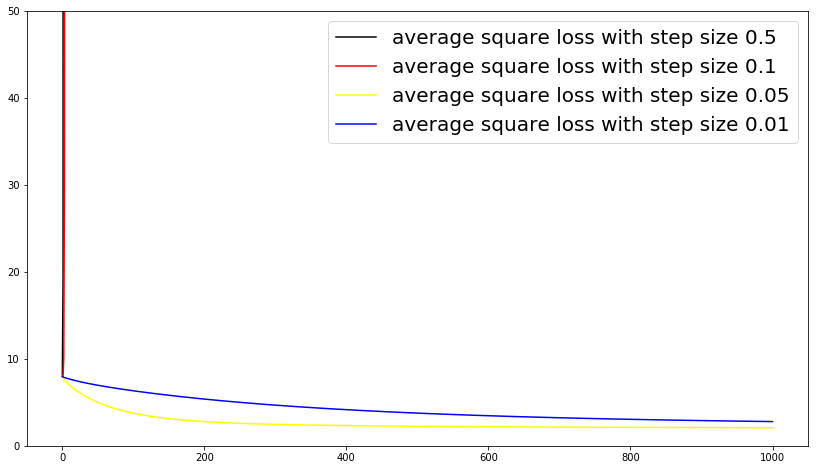
\includegraphics[scale=0.6]{342.png}
As we can see from the plot, when step size is too large(like 0.1, 0.5), the gradient descent does not converge, when step size is less than a relatively small value, gradient descent converges. And it converges slower when step size is smaller.
\endsubsection

\subsection{3.4.3 backtracking line search}
\begin{minted}[mathescape,
               linenos,
               numbersep=5pt,
               gobble=2,
               frame=lines,
               framesep=2mm]{csharp}
  def batch_grad_descent_backtracking(X, y, step=1, alpha=0.25, beta = 0.8,num_step=1000, grad_check=False):
    num_instances, num_features = X.shape[0], X.shape[1]
    theta_hist = np.zeros((num_step+1, num_features)) #Initialize theta_hist
    loss_hist = np.zeros(num_step+1) #Initialize loss_hist
    theta = np.zeros(num_features) #Initialize theta
    
    #TODO
    loss_hist[0] = skeleton_code.compute_square_loss(X, y, theta) # initial loss
    theta_hist[0] = theta # initial theta
    for i in range(num_step):
        grad = skeleton_code.compute_square_loss_gradient(X, y, theta)
        left = skeleton_code.compute_square_loss(X,y,(theta-step*grad)) 
        right = skeleton_code.compute_square_loss(X,y, theta) - alpha*step*
        (np.linalg.norm(grad)**2)
        if left > right:
            step = beta * step
        theta = theta - step * grad
        theta_hist[i + 1] = theta
        loss = skeleton_code.compute_square_loss(X, y, theta)
        loss_hist[i + 1] = loss
    return theta_hist, loss_hist
    
    _,loss_hist1 = batch_grad_descent_backtracking(X_train, y_train, step=1, alpha=0.25,
    beta = 0.8,num_step=1000, grad_check=False)
    plt.plot(loss_hist1, label = 'step size adjusted by backtracking line search')
    theta_hist3, loss_hist3 = skeleton_code.batch_grad_descent(X_train, y_train, alpha=0.05,
    num_step=1000, grad_check=False)
    theta_hist4, loss_hist4 = skeleton_code.batch_grad_descent(X_train, y_train, alpha=0.01,
    num_step=1000, grad_check=False)
    plt.plot(loss_hist3, label = 'average square loss with step size 0.05')
    plt.plot(loss_hist4, label = 'average square loss with step size 0.01')
    plt.ylim(0,20)
    plt.ylabel('average square loss')
    plt.xlabel('num of steps')
    plt.legend()
    # plt.savefig('343.png')
    plt.show()
    
    %timeit skeleton_code.batch_grad_descent_backtracking(X_train, y_train, step=1, alpha=0.25, beta = 0.8,num_step=1000, grad_check=False)
    %timeit skeleton_code.batch_grad_descent(X_train, y_train, alpha=0.05, num_step=1000, grad_check=False)
\end{minted}
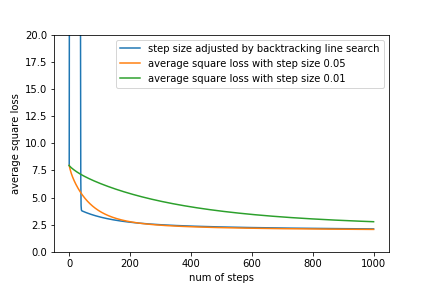
\includegraphics[scale=1.2]{343.png}
Compared to fixed steps, backtracking line search can help us get to the minimum point much faster, and its effect is of no apparent difference with the best fixed step-size I found in the previous question.
The time that gradient descent using backtracking line search spends is :
47.2 ms ± 2.2 ms per loop (mean ± std. dev. of 7 runs, 10 loops each).
And the one without backtracking line search is:
18.4 ms ± 751 µs per loop (mean ± std. dev. of 7 runs, 10 loops each).
So extra time to run backtracking line search is around 1.5 times of the time it takes to compute the gradient.
\endsubsection

\section{3.5 Ridge Regression}
\subsection{3.5.2}
\begin{minted}[mathescape,
               linenos,
               numbersep=5pt,
               gobble=2,
               frame=lines,
               framesep=2mm]{csharp}
  
  def compute_regularized_square_loss_gradient(X, y, theta, lambda_reg):
    """
    Compute the gradient of L2-regularized average square loss function given X, y and theta

    Args:
        X - the feature vector, 2D numpy array of size (num_instances, num_features)
        y - the label vector, 1D numpy array of size (num_instances)
        theta - the parameter vector, 1D numpy array of size (num_features)
        lambda_reg - the regularization coefficient

    Returns:
        grad - gradient vector, 1D numpy array of size (num_features)
    """
    #TODO
    num_instances, num_features =  X.shape[0],X.shape[1]
    factor = np.matmul(X,theta) - y
    grad = 2/num_instances * np.matmul(X.transpose(), factor) + 2 * lambda_reg * theta
    return grad
\end{minted}

\subsection{3.5.3}
\begin{minted}[mathescape,
               linenos,
               numbersep=5pt,
               gobble=2,
               frame=lines,
               framesep=2mm]{csharp}
  def regularized_grad_descent(X, y, alpha=0.05, lambda_reg=10**-2, num_step=1000):
    """
    Args:
        X - the feature vector, 2D numpy array of size (num_instances, num_features)
        y - the label vector, 1D numpy array of size (num_instances)
        alpha - step size in gradient descent
        lambda_reg - the regularization coefficient
        num_step - number of steps to run
    
    Returns:
        theta_hist - the history of parameter vector, 2D numpy array of size (num_step+1, num_features)
                     for instance, theta in step 0 should be theta_hist[0], theta in step (num_step+1) is theta_hist[-1]
        loss hist - the history of average square loss function without the regularization term, 1D numpy array.
    """
    num_instances, num_features = X.shape[0], X.shape[1]
    theta = np.zeros(num_features) #Initialize theta
    theta_hist = np.zeros((num_step+1, num_features)) #Initialize theta_hist
    loss_hist = np.zeros(num_step+1) #Initialize loss_hist
    #TODO
    loss_hist[0] = compute_square_loss(X, y, theta) + 
    lambda_reg * np.matmul(theta.transpose(), theta) # initial loss
    theta_hist[0] = theta
    for i in range(num_step):
        grad = compute_regularized_square_loss_gradient(X, y, theta, lambda_reg)
        theta = theta - alpha * grad
        theta_hist[i + 1] = theta
        loss = compute_square_loss(X, y, theta) + lambda_reg * np.matmul(theta.transpose(),
        theta)
        loss_hist[i + 1] = loss
    return theta_hist,loss_hist
\end{minted}
\endsubsection

\subsection{3.5.7}
\begin{minted}[mathescape,
               linenos,
               numbersep=5pt,
               gobble=2,
               frame=lines,
               framesep=2mm]{csharp}
    import matplotlib.pyplot as plt
    %matplotlib inline
    %config InlineBackend.figure_format = 'svg'
    fig = plt.gcf()
    fig.set_size_inches(12, 4)
    def loss_lambda(lambda_list):
    loss_train_list = []
    loss_test_list = []
    for lambda_reg in lambda_list:
        lambda_reg = 10**(lambda_reg)
        theta_hist1, loss_hist1 = skeleton_code.regularized_grad_descent(X_train,y_train,0.05,lambda_reg,1000)
        theta = theta_hist1[-1]
        loss_train = skeleton_code.compute_square_loss(X_train, y_train, theta) 
        loss_train_list.append(loss_train)
        loss_test = skeleton_code.compute_square_loss(X_test, y_test, theta) 
        loss_test_list.append(loss_test)
    plt.plot(lambda_list,loss_train_list,color = 'black', label = 'average square loss_training')
    plt.plot(lambda_list,loss_test_list,color = 'blue', label = 'average square loss_test')
 
    plt.subplot(1,2,1)
    lambda_list = [-7,-5,-3,-1,0,1,2]
    loss_lambda(lambda_list)
    plt.legend()
    plt.ylim(0,10)
    plt.xlabel('log($\lambda$)')
    plt.ylabel('Average Square Loss')
    
    plt.subplot(1,2,2)
    lambda_list = np.linspace(-3,-1,num = 50)
    loss_lambda(lambda_list)
    plt.legend()
    plt.ylim(0,10)
    plt.xlabel('log($\lambda$)')
    plt.ylabel('Average Square Loss')
    plt.show()
\end{minted}
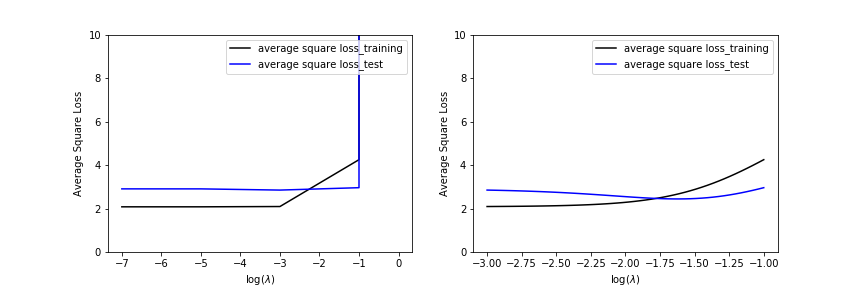
\includegraphics[scale=0.6]{357.png}

\endsubsection

\section{3.6 Stochastic Gradient Descent}
\subsection{3.6.4; 3.6.5}
\begin{minted}[mathescape,
               linenos,
               numbersep=5pt,
               gobble=2,
               frame=lines,
               framesep=2mm]{csharp}
  def stochastic_grad_descent(X, y, alpha=0.01, lambda_reg=10**-2, num_epoch=1000,C=0.1):
    """
    In this question you will implement stochastic gradient descent with regularization term

    Args:
        X - the feature vector, 2D numpy array of size (num_instances, num_features)
        y - the label vector, 1D numpy array of size (num_instances)
        alpha - string or float, step size in gradient descent
                NOTE: In SGD, it's not a good idea to use a fixed step size. Usually it's set to 1/sqrt(t) or 1/t
                if alpha is a float, then the step size in every step is the float.
                if alpha == "1/sqrt(t)", alpha = 1/sqrt(t).
                if alpha == "1/t", alpha = 1/t.
                t = num steps = (num epochs) x (num instances)
        lambda_reg - the regularization coefficient
        num_epoch - number of epochs to go through the whole training set

    Returns:
        theta_hist - the history of parameter vector, 3D numpy array of size (num_epoch, num_instances, num_features)
                     for instance, theta in epoch 0 should be theta_hist[0], theta in epoch (num_epoch) is theta_hist[-1]
        loss hist - the history of loss function vector, 2D numpy array of size (num_epoch, num_instances)
    """
    num_instances, num_features = X.shape[0], X.shape[1]
    theta = np.ones(num_features) #Initialize theta

    theta_hist = np.zeros((num_epoch, num_instances, num_features)) #Initialize theta_hist
    loss_hist = np.zeros((num_epoch, num_instances)) #Initialize loss_hist
    #TODO
    loss_hist[0] = skeleton_code.compute_square_loss(X, y, theta_hist[0][0]) #initial loss
    
    t = 0
    for i in range(num_epoch):
        #shuffle data
        idx = np.arange(num_instances)
        np.random.shuffle(idx)
        X = X[idx]
        y = y[idx] 
        for j in range(num_instances):
            t = t+1
            if alpha =='1/sqrt(t)':
                step_size = C/(t**(1/2))
            elif alpha == '1/t':
                step_size = C/t
            else:
                step_size = alpha
            factor = np.matmul(X[j],theta) -  y[j]  #h(xi) - y(i)
            theta = theta - 2 * step_size * (factor * X[j].transpose() + lambda_reg * theta)
            theta_hist[i][j] = theta   
            loss_hist[i][j] = skeleton_code.compute_square_loss(X,y,theta) + lambda_reg * 
            np.matmul(theta.transpose(), theta)
            
    return theta_hist, loss_hist 
\end{minted}
\begin{center}
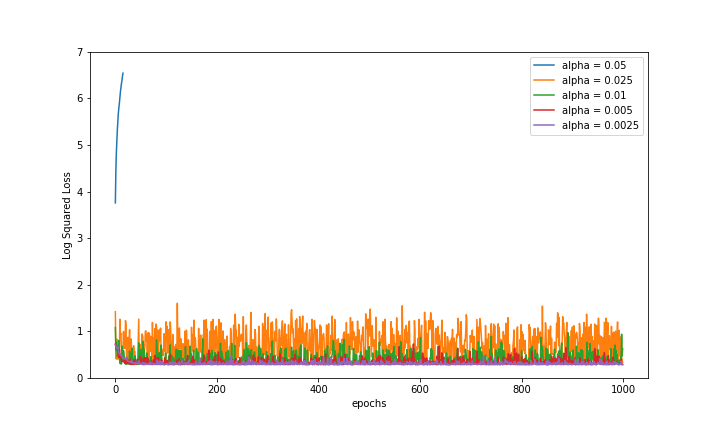
\includegraphics[scale=0.6]{3651.png}
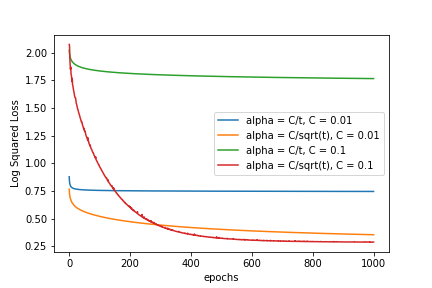
\includegraphics[scale=0.9]{3652.png}
\end{center}
From the above figures, we can see that when step size is fixed, gradient descent doesn't converge when it's too big(eg. alpha = 0.05), when step size is smaller than some value, it will converge much more faster than batch gradient descent, but the loss function is much more fluctuating. Because SGD's convergence is much slower than GD once it get closer to the minimizer. And SGD will be less volatile when step size is smaller because once step size is smaller enough, the update of the loss will be mild(eg. the curve is less fluctuating when alpha = 0.0025 than alpha = 0.025).
When we use step sizes that decrease with the step number according to certain rules mentioned in the question, we found that the loss function became much smoother and when rule is "C/sqrt(t)", the loss function converges slower, and loss function with larger C in step size converges to larger loss.
\endsubsection 

\subsection{3.6.6}
\begin{minted}[mathescape,
               linenos,
               numbersep=5pt,
               gobble=2,
               frame=lines,
               framesep=2mm]{csharp}
  def stochastic_grad_descent_newrule(X, y, step, lambda_reg=10**-2, num_epoch=1000):
    num_instances, num_features = X.shape[0], X.shape[1]
    theta = np.ones(num_features) #Initialize theta
    theta_hist = np.zeros((num_epoch, num_instances, num_features)) #Initialize theta_hist
    loss_hist = np.zeros((num_epoch, num_instances)) #Initialize loss_hist
    #TODO  
    loss_hist[0] = skeleton_code.compute_square_loss(X, y, theta_hist[0][0]) #initial loss
    t = 0  
    for i in range(num_epoch):
        idx = np.arange(num_instances)
        np.random.shuffle(idx)
        X = X[idx]
        y = y[idx]
        for j in range(len(X)):
            t = t+1
            factor = np.matmul(X[j],theta) -  y[j]  #h(xi) - y(i)
            theta = theta - 2 * step * (factor * X[j].transpose() + lambda_reg * theta)
            step = step/(1+ step*lambda_reg*t)
            theta_hist[i][j] = theta   
            loss_hist[i][j] = skeleton_code.compute_square_loss(X,y,theta) + 
            lambda_reg * np.matmul(theta.transpose(), theta)
    return theta_hist, loss_hist               
\end{minted}
\begin{center}
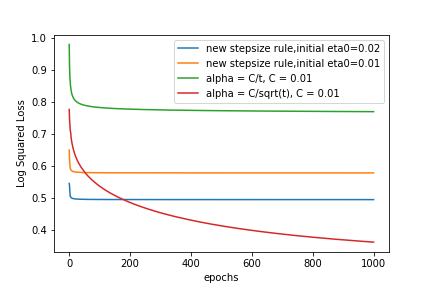
\includegraphics[scale=0.6]{366.png}
\end{center}
Compared to the previous curve, we found that this new rule can help converge faster but the minimum of loss it can get is not as good as 'C/sqrt(t)'.
\end{document}
